\chapter{Tools}\label{ch02:00}

\myepigraph{The expectations of life depend upon diligence; the mechanic that would perfect his work must first sharpen his tools.}{Confucius}

  The platform can be used for developing software using any IDE for Java such as IntelliJ IDEA or Netbeans.
  However, the recommended IDE for this is Eclipse due to provided set of plugins developed specifically to facilitate TG-based development.
  
\section{Eclipse Plugins}

  The main features that are provided by the developed plugin pertain to automating creation of fractal objects, main menu items and UI.
  The provided automation is easily comparable to that provided by inbuilt Delphi features such as creation of forms and data modules.
  
  The plugin is distributed in a from of a jar file \texttt{tg-eclipse-plugin\_\textless version\textgreater.jar}.
  It can be installed by placing the jar into Eclipses \texttt{dropins} directory.
  Once installed, the plugin integrates with the \emph{Package Explorer} context menu.
  
  There are three groups of actions that can be invoked from a context menu:
  
  \begin{description}
    \item[\textbf{TG Model Actions.}] Represents actions that facilitate creation of different kinds of entity types.
    Fig.~\ref{img:ch02:00:model-actions} depicts the menu.
    
    \begin{itemize}
     \item \emph{Create Master Entity/Companion Objects\ldots} -- generates a pair of master entity and companion objects with respective DAO and RAO default implementations for the companion object.
     \item \emph{Create One-2-One Entity/Companion Objects\ldots} -- generates a pair of entity and companion objects with respective DAO and RAO default implementations for the companion object: the generated entity models a one-2-one relationship with a master entity, which gets specified during creation.
     \item \emph{Create One-2-Many Entity/Companion Objects\ldots} -- generates a pair of entity and companion objects with respective DAO and RAO default implementations for the companion object; the generated entity models a one-2-many relationship with a master entity, which gets specified during creation.
    \end{itemize}

    \begin{image}{Entity model creation actions.}{\label{img:ch02:00:model-actions}}
      \begin{tikzpicture}[remember picture, >=latex', note/.style={rectangle callout, rounded corners = 1pt, fill=annotationbgcolor, drop shadow}]
	\pgftext{%
	    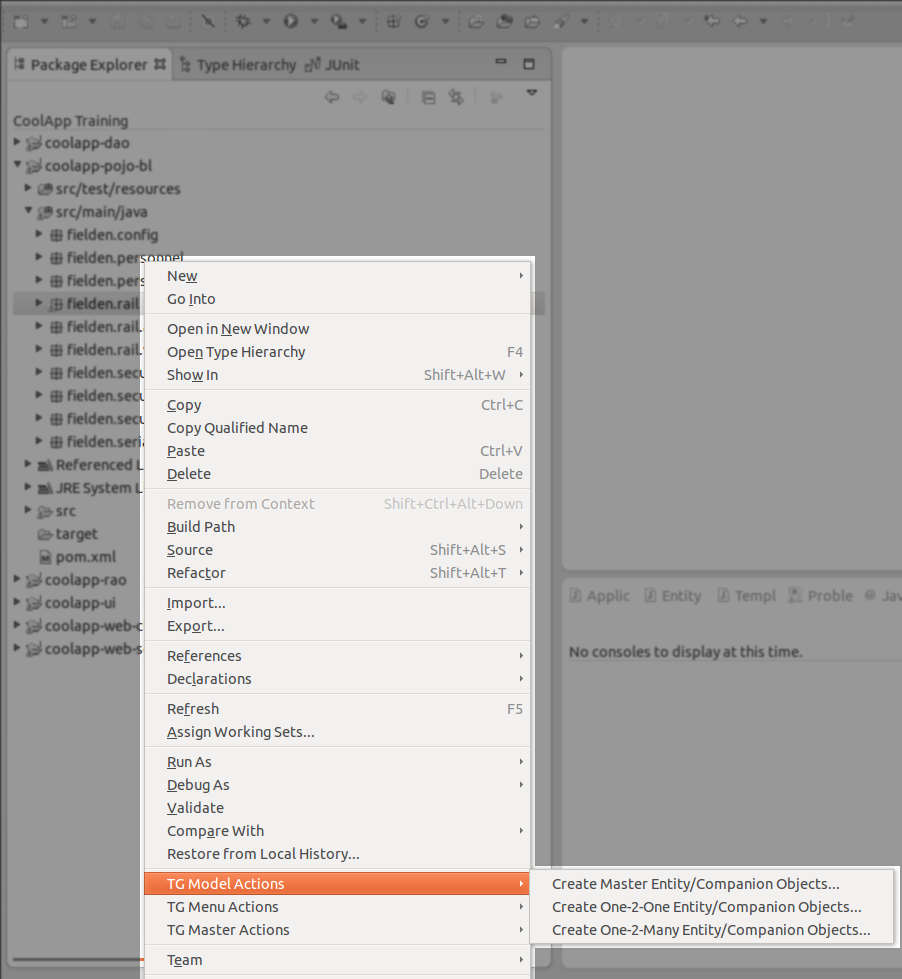
\includegraphics[width=0.6\textwidth]{parts/02-part/chapters/00-tools/images/01-tg-model-actions.png}
	}%

	\node [overlay, note=annotationbgcolor, callout absolute pointer={(-4,1.8)}] at (-6.5,3.5) 
	{
	  \begin{minipage}{3cm}
	  \tiny
	  \textbf{Package Explorer}\newline
	  The actions are integrated into the context menu of Package Explorer.
	  \end{minipage}
	};

	\node [overlay, note=annotationbgcolor, callout absolute pointer={(2,-3.8)}] at (5,-2.5) 
	{
	  \begin{minipage}{3cm}
	  \tiny
	  \textbf{Subitem}\newline
	  Three actions for creating different kinds of entity objects.
	  \end{minipage}
	};
      \end{tikzpicture}  
    \end{image}
    
    
    \item[\textbf{TG Menu Actions.}] Represents actions that facilitate creation of the application main menu items.
    Fig.~\ref{img:ch02:00:menu-actions} depicts the menu.
    
    \begin{itemize}
     \item \emph{Create Group Menu\ldots} -- generates a menu item that can be used for grouping of sub-items.
     \item \emph{Create Simple Menu} -- generates the most trivial menu item for a selected entity that gets associated with a centre for that entity.
     \item \emph{Create Menu Entry with Custom Command} -- generates a menu items for a selected entity that gets associated with a centre for that entity, and provides a stub for a custom action.
    \end{itemize}

    \begin{image}{Menu Actions.}{\label{img:ch02:00:menu-actions}}
      \begin{tikzpicture}[remember picture, >=latex', note/.style={rectangle callout, rounded corners = 1pt, fill=annotationbgcolor, drop shadow}]
	\pgftext{%
	  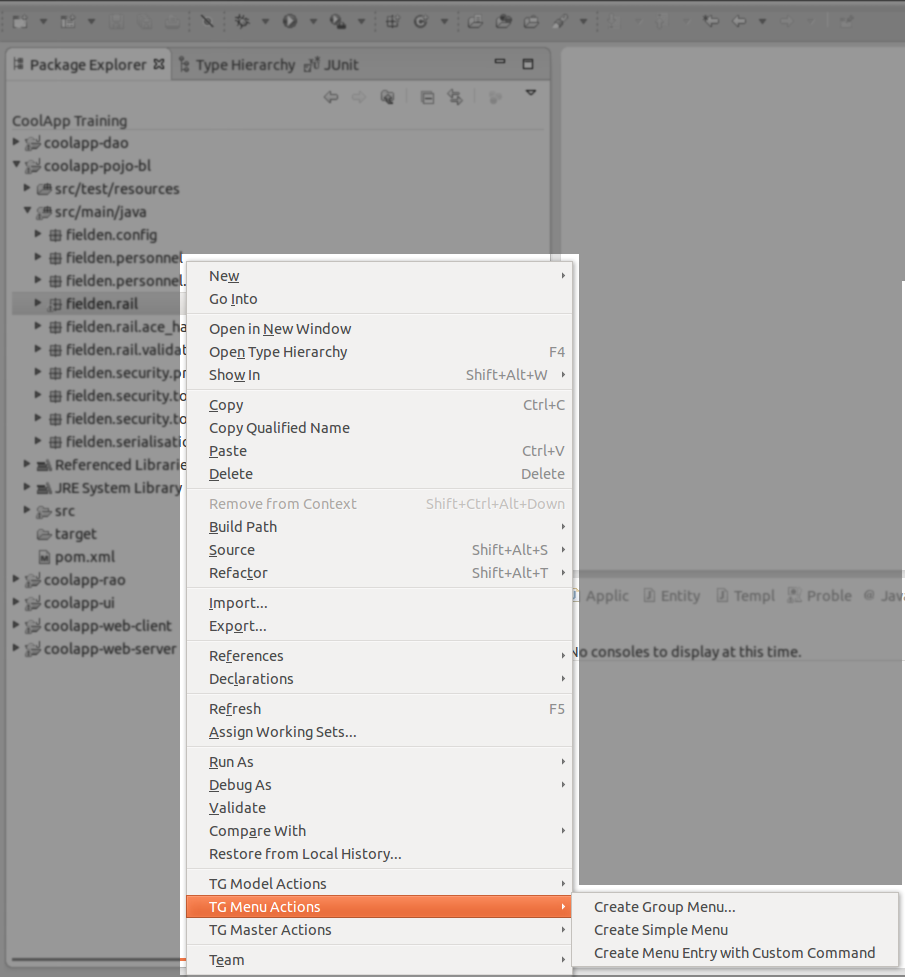
\includegraphics[width=0.6\textwidth]{parts/02-part/chapters/00-tools/images/02-tg-menu-actions.png}
	}%

	\node [overlay, note=annotationbgcolor, callout absolute pointer={(-4,1.8)}] at (-6.5,3.5) 
	{
	  \begin{minipage}{3cm}
	  \tiny
	  \textbf{Package Explorer}\newline
	  The actions are integrated into the context menu of Package Explorer.
	  \end{minipage}
	};

	\node [overlay, note=annotationbgcolor, callout absolute pointer={(2,-4.0)}] at (5,-2.5) 
	{
	  \begin{minipage}{3cm}
	  \tiny
	  \textbf{Subitem}\newline
	  Three actions for creating different kinds of application main menu items.
	  \end{minipage}
	};
      \end{tikzpicture}  
    \end{image}
    
    \item[\textbf{TG Master Actions.}] Represents actions that facilitate creation of various kinds of entity master forms that are used as a front end for creation and modification of entity instances. 
    Fig.~\ref{img:ch02:00:master-actions} depicts the menu.
    
    \begin{itemize}
     \item \emph{Create Simple Master for Entity} -- generates a pair of UI model and view that represent an simple entity master form; suitable for entities that do not have (or do not require) one-2-many associations.
     \item \emph{Create Compound Master for Entity} -- generates UI (a model and two views) that assumes a master form with a tree menu, where each menu item (except the first) represents some association for a selected during generation entity; only the first item menu item is generated that gets associated with a view for entry and modification of non-collectional entity properties (one can think of it as main entity data).
     \item \emph{Create Compound Master Sub Model/View for Entity (One-2-One)\ldots} -- generates a pair of UI sub-model and sub-view that should be associated with some compound master; this UI pair is generated for an entity that is in one-2-one association to some master entity object; the UI provides means to create and modify instances of the subordinate entity object with automatic association to a corresponding master entity object.
     \item \emph{Create Compound Master Sub Model/View for Entity (One-2-Many)\ldots} -- generates a pair of UI sub-model and sub-view that should be associated with some compound master; this UI pair is generated for an entity that is in one-2-many association to some master entity object; the UI provides means to create and modify multiple instance of the subordinate entity object with automatic association to a corresponding master entity object.
     \item \emph{Create Compound Master Sub Model/View for Entity (One-2-Many Centre-Based)\ldots} -- generates a pair of UI sub-model and sub-view that resembles an entity centre where selection criteria section is configured at the source level; this kind of UI also supports customisation of the toolbar by providing custom actions; the resultant from such model queries are automatically enhanced with a filtering condition to show only instances that are associated with a corresponding master entity object.
     \item \emph{Create Entity Producer with User} -- generates an entity producer that gets used for creation of new entity instances on master forms; the generated producer contains the code for obtaining system user at runtime, which comes handy when new entities should be initialised with the information about their creator.
    \end{itemize}

    \begin{image}{Master Actions.}{\label{img:ch02:00:master-actions}}
      \begin{tikzpicture}[remember picture, >=latex', note/.style={rectangle callout, rounded corners = 1pt, fill=annotationbgcolor, drop shadow}]
	\pgftext{%
	  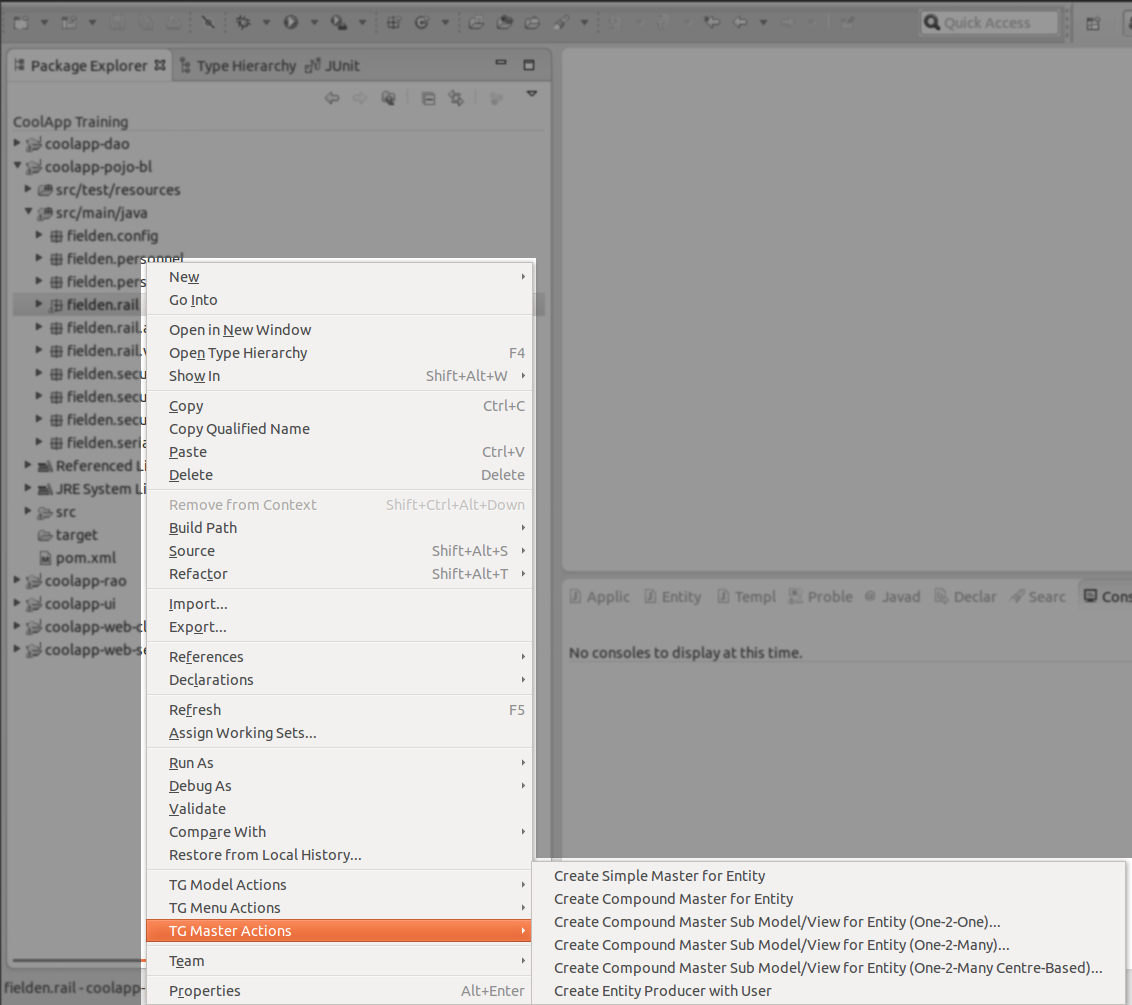
\includegraphics[width=0.6\textwidth]{parts/02-part/chapters/00-tools/images/03-tg-master-actions.png}
	}%

	\node [overlay, note=annotationbgcolor, callout absolute pointer={(-4,1.8)}] at (-6.5,3.5) 
	{
	  \begin{minipage}{3cm}
	  \tiny
	  \textbf{Package Explorer}\newline
	  The actions are integrated into the context menu of Package Explorer.
	  \end{minipage}
	};

	\node [overlay, note=annotationbgcolor, callout absolute pointer={(2,-2.8)}] at (5,-0.5) 
	{
	  \begin{minipage}{3cm}
	  \tiny
	  \textbf{Subitem}\newline
	  Actions for creating UI artefacts such as models and views for entity master forms, entity producers used by master forms.
	  \end{minipage}
	};
      \end{tikzpicture}  
    \end{image}
    
    
  \end{description}

  Some of the actions should be invoked on specific classes or packages, and generate associated with them artefacts without any additional parameters.
  However, other actions bring up wizards that require specific inputs, and only once those inputs are populated, can be used to generated associated artefacts.
  Some of the inputs get populated based on the invocation context (e.g. package name can be populated if the context menu was invoked on a package).
  The following subsections delves more into the details about specific plugin actions.

  \subsection{Creation of Entity Objects}

  As has been discussed in section~\ref{ch01:02} all entity objects can be distilled down to three principle kinds:
  
  \begin{itemize}
   \item Master entity;
   \item Subordinate one-2-one entity that gets associated with a single master entity;
   \item Subordinate one-2-many entity where one or more instances get associated with a single master entity.
  \end{itemize}

  In reality the situation could get a lot more complex as any of the one-2-one and one-2-many kinds may act in turn as master entities to other subordinate types. 
  This is, however, only natural if the domain inherently requires such complexity.  
  Thus, there are three actions -- one for creating each kind of an entity object.
  
  The master entity together with its companion object can be created using action \emph{Create Master Entity/Companion Objects\ldots}.
  Fig.~\ref{img:ch02:00:model-actions-new-master-entity-01} depicts a wizard window that gets displayed upon action invocation.
  It is most natural for this action to be invoked on a package within the pojo-bl application module where an intended entity object should reside.
  This way the plugin automatically populates the package entry as illustrated in Fig.~\ref{img:ch02:00:model-actions-new-master-entity-01}.
  Otherwise, the package should be specified.
  
  Most of the options in this wizard are described in Fig.~\ref{img:ch02:00:model-actions-new-master-entity-01}.
  However, the provided checkbox options require a little bit more explanation:
  \begin{description}
   \item[\textbf{should have property 'desc'}] -- 
   specifies whether entity object should have the description property; most entities requires or may use such property as comes at no cost; 
   presence or absence of property \texttt{desc} is controlled via annotation \texttt{@DescTitle}; 
   if this annotation is not declared as part of entity object definition then property \texttt{desc} is recognised by the platform as absent;

   \item[\textbf{should be persistent}] -- 
   if a synthesised or a functional entity needs to be created then this option should be unchecked; such entities do not usually have a persistent state; 
   however, if a persistent entity needs to be created then this option should be left on; from our experience the number of persistent entities is significantly greater than that of synthesised or a functional entities, thus by default this option if on;

   \item[\textbf{use mixin for common RAO/DAO code}] -- 
   often methods in RAO and DAO that implement companion object contract have exactly the same implementation\footnote{This happens mainly due to the universal execution model for CRUD operations (including EQL queries) that works seamlessly at both the client and server sides.)}; 
   in order to avoid code duplication to improve system maintainability, it makes sense to place the common for RAO and DAO methods into a single class that could be than reused in both places; 
   the platform provides a convenient support for this in a form of a \emph{\href{http://en.wikipedia.org/wiki/Mixin}{mixin}} -- a class that should contains common methods and has a companion object (an interface) as its constructor argument; such mixin can be naturally mixed into both RAO and DAO implementations by means of composition; 
   if this option is selected then a mixin class would get generated and integrated into the RAO and DAO classes that also get generated as part of entity object creation;

   \item[\textbf{support deletion}] -- 
   many, especially persistent entities, may require deletion support; 
   by default deletion is disabled at the base level of the common companion object ancestor that is provided by the platform, and needs to be enabled explicitly by overriding corresponding methods; 
   in most cases deletion is safe due to automatic management of dependencies between entities, but due to severity of such action by default it is disabled; 
   this option should be selected if support for deletion is required for the entity being created.
  \end{description}
 
  \begin{image}{Create Master Entity/Companion Objects.}{\label{img:ch02:00:model-actions-new-master-entity-01}}
    \begin{tikzpicture}[remember picture, >=latex', note/.style={rectangle callout, rounded corners = 1pt, fill=annotationbgcolor, drop shadow}]
      \pgftext{%
	  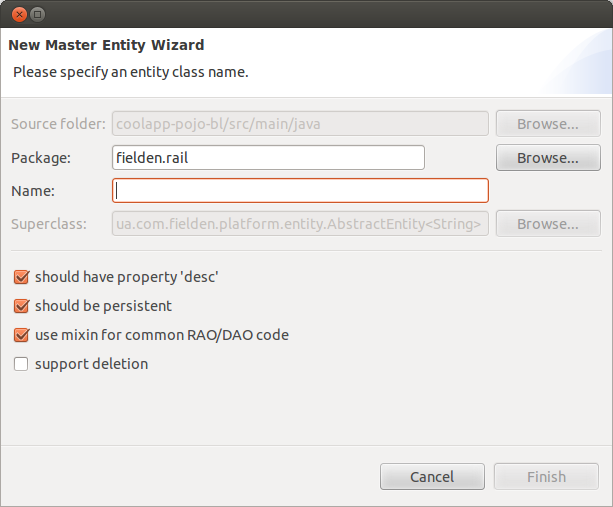
\includegraphics[width=0.6\textwidth]{parts/02-part/chapters/00-tools/images/01-01-new-master-entity.png}
      }%

      \node [overlay, note=annotationbgcolor, callout absolute pointer={(-4,2.0)}] at (-6.5,3.5) 
      {
	\begin{minipage}{3cm}
	\tiny
	\textbf{Source folder}\newline
	Regardless of where the context menu is invoked, the source folder is identified automatically and always points to the pojo-bl module of the application.
	\end{minipage}
      };
      
      \node [overlay, note=annotationbgcolor, callout absolute pointer={(-4.3,1.4)}] at (-6.5,1.0) 
      {
	\begin{minipage}{3cm}
	\tiny
	\textbf{Package name}\newline
	If the action is selected from a context menu that was invoked on a package then the package name gets populated automatically.
	Otherwise it needs to be specified manually or selected for a dialog that is accessible via button \emph{Browse}.
	\end{minipage}
      };
      

      \node [overlay, note=annotationbgcolor, callout absolute pointer={(2.0,1.0)}] at (5.0,3.1) 
      {
	\begin{minipage}{3cm}
	\tiny
	\textbf{Name}\newline
	This is a class name that should adhere to camel case naming convention.
	It is used as the name for a class representing an entity object.
	\end{minipage}
      };      

      \node [overlay, note=annotationbgcolor, callout absolute pointer={(2.0,0.5)}] at (7.0,1.0) 
      {
	\begin{minipage}{4cm}
	\tiny
	\textbf{Superclass}\newline
	All entity objects are descendant of class \texttt{AbstractEntity}.
	The assumed key type for master entity is \texttt{String} with \texttt{Integer} as an option that could be specified one classes are created.	
	\end{minipage}
      };      

      \node [overlay, note=annotationbgcolor, callout absolute pointer={(0,-0.7)}] at (4,-1) 
      {
	\begin{minipage}{4cm}
	\tiny
	\textbf{Options}\newline
	Provides support for customising an entity being generated.
	More details about each option are outlined in the text.
	\end{minipage}
      };
    \end{tikzpicture}  
  \end{image}
  
  Once all the required inputs are populated, button \emph{Finish} becomes enabled.
  Pressing it leads to the generation of a number of classes and interfaces that together represent an entity object, a companion object, RAO and DAO implementations for a companion object, and a mixin class (depending on options selected).
  At the end, the wizard produces a warning advising the developer to register the generated entity type as part of the application domain.
  This is done by calling static method \texttt{add} with the class for entity object as an argument in the static initialisation block of class \texttt{ApplicationDomain}.
  Every TG-based application is provided with class \texttt{ApplicationDomain}, and the place where new entities should registered becomes obvious once \texttt{ApplicationDomain} is open in the code editor.
  
  In order to describe the generated artefacts let's consider a concrete example based on our illustrative application \emph{collapp}.
  Let the name of the generated master entity be \texttt{Bogie}, and let's also consider that its package is \texttt{fielden.rail} and that all options on the entity wizard have been selected (including deletion and mixin options).
  Fig.~\ref{img:ch02:00:model-actions-new-master-entity-artefacts} depicts a UML diagram that specifies all classes that are generated and their location in terms of packages and application modules.
  
  \begin{image}{Create Master Entity/Companion Objects Artefacts.}{\label{img:ch02:00:model-actions-new-master-entity-artefacts}}    
    \scalebox{1.0} {
    \begin{tikzpicture}
      \draw[very thick, dashed, color=blue!50!black, rounded corners] (-2.3, 2.5) rectangle (3.0,-1.5);
      \node[rotate=90,color=blue!50!black] at (-2.6, 1.5) {\small coolapp-dao};
      
      \begin{umlpackage}[x=0,y=0]{fielden-rail} 
        \umlemptyclass[x=0,y=0,template={Bogie}]{BogieDao}
      \end{umlpackage}
      
      
      \draw[very thick, dashed, color=red!50!black, rounded corners] (3.5, 2.0) rectangle (11.0,-3.0);
      \node[color=red!50!black] at (9.5, 2.3) {\small coolapp-pojo-bl};
      \begin{umlpackage}[x=6.0,y=-1]{fielden-rail}       
        \umlemptyclass[x=0,y=0,template={Bogie},type=interface]{IBogie}
        \umlemptyclass[x=3,y=0]{Bogie}
      \end{umlpackage}      
      
    \end{tikzpicture}
    }
  \end{image}  

%       \umlbasiccomponent[x=8, y=0, fill=blue!10]{coolapp-web-server}
% 
%       \draw[very thick, dashed, color=red!50!black, rounded corners] (1.8, -3.3) rectangle (6.2,-6.1);
%       \node[color=red!50!black] at (4.9, -3) {\small Shared Module};
%       \umlbasiccomponent[x=4, y=-5]{coolapp-pojo-bl}
%       
%       \umlnote[x=-2, y=3.5, width=5.5cm, fill=annotationbgcolor]{coolapp-dao}{\scriptsize Date Access Objects layer, which provides RDBMS-based implementation for domain controllers.}
%       \umlnote[x=-2, y=-3.5, width=5.5cm, fill=annotationbgcolor]{coolapp-pojo-bl}{\scriptsize Defines business domain model (entities and controllers), shared between client and server tiers.}
% 
%       \umluniassoc{coolapp-dao}{coolapp-pojo-bl}
%       \umluniassoc[name=w2d]{coolapp-web-server}{coolapp-dao}
%       \umlnote[x=5, y=3.5, width=5.5cm, fill=annotationbgcolor]{w2d-1}{\scriptsize Web resources use DB driven implementation of domain controllers} 
% 
%       \draw[very thick, dashed, color=green!50!black, rounded corners] (-1, -8.1) rectangle (8.9,-15.2);
%       \node[rotate=90,color=green!50!black] at (-1.3, -9.7) {\small Client Modules};
% 
%       \umlbasiccomponent[x=7, y=-10, fill=green!30]{coolapp-ui}
%       \umlbasiccomponent[x=1, y=-10, fill=green!30]{coolapp-rao}
%       \umlbasiccomponent[x=4, y=-14, fill=green!30]{coolapp-web-client}   
% 
%       \umlnote[x=-2, y=-6.5, width=5.5cm, fill=annotationbgcolor]{coolapp-rao}{\scriptsize Resource Access Objects, which provides HTTP-based implementation for domain controllers.}
%       \umlnote[x=-3, y=-13.7, width=3cm, fill=annotationbgcolor]{coolapp-web-client}{\scriptsize Binds together UI and RAO implementation of domain controllers to define a web client application.}
% 
%       \umluniassoc[name=u2m]{coolapp-ui}{coolapp-pojo-bl}
%       \umlnote[x=9, y=-6, width=3.5cm, fill=annotationbgcolor]{u2m-1}{\scriptsize Accessed domain model and controller via their contracts (not implementation).} 
%       \umluniassoc{coolapp-rao}{coolapp-pojo-bl}
%       \umluniassoc{coolapp-web-client}{coolapp-ui}
%       \umluniassoc{coolapp-web-client}{coolapp-rao}  
  
  
  
  \subsection{Creation of Main Menu Items and Entity Centres}
  
  
  \subsection{Creation Entity Masters}
  
